\autoref{fig:bearing} shows that the \ac{TM} can be positioned at various distances and angles in relation to the \ac{FH}.
For one corn harvest scenario, \textcite{klingler_agriculture_2018} found out that the \ac{RSS} can drop due to
shadowing effects caused by the size and shape of the \ac{FH} and the \ac{TM}.

In a field experiment, I want to analyze which positions of the \ac{TM} and \ac{FH} cause the shadowing effects which
subsequently reduce the \ac{RSS}, and how physical layer parameters like \ac{MCS} and \ac{STBC} can used to ensure a low
\ac{PER}.

For the experiment, I will use a \ac{CH} instead of a \ac{FH} as it has a similar shape and size as a \ac{FH} and is available.
The \ac{TM} will be a Tractor pulling a trailer of the type HW80.
Both machines will be equipped with a \ac{GPS} receiver and Wi-Fi devices which record the position, \ac{RSS} and the \ac{PER} of the
exchanged packets.
The \ac{CH} will be positioned in an agricultural field.
The tractor will start \SI{50}{\metre} behind the \ac{CH}, advance to the \ac{CH} and pass the \ac{CH} slowly with a
speed of \SIrange{1}{5}{\kilo\metre\per\hour} (\SIrange{0.28}{1.39}{\metre\per\second}) as shown in \autoref{fig:fieldDrive}.
\begin{figure}[]%
	\centering
	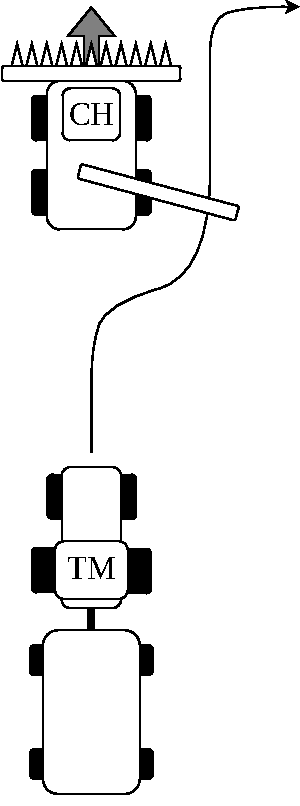
\includegraphics[width=0.21\textwidth]{figures/FieldExperimentDrive}
	\caption{Path around the static \acf{CH}, which the \acf{TM} will drive during the experiment to mimic various overloading positions}%
	\label{fig:fieldDrive}
\end{figure}

While driving along the specified path, the tractor will mimic various overloading positions, where shadowing effects can occur. After the tractor has passed the \ac{CH},
it will drive back to its starting position, and the experiment will be repeated with different overloading distances between the \ac{CH} and the tractor.

During the experiments, \ac{GPS} receivers at the agricultural machines will record the position and speed of the machines every \SI{1}{\second}.

The Wi-Fi setup consists of a Milesight Industrial Router UR75 \footnote{\url{https://iot-shop.de/en/shop/mil-ur75-500gl-g-p-w-milesight-ur75-500gl-g-p-w-industrial-cellular-5g-router-with-gps-wifi-and-poe-5677}}, which implements the standards IEEE 802.11 b/g/n in the \SI{2.4}{\giga\hertz} band and IEEE 802.11 a/n/ac in the \SI{5}{\giga\hertz} band and
IEEE 802.11 a/n/ac in the \SI{5}{\giga\hertz} band.
The router is equipped with two omnidirectional antennas for  \SI{2.4}{\giga\hertz} and \SI{5}{\giga\hertz} usage.
\textcite{brinkhoff_characterization_2017} and \textcite{paul_characterizing_2011}  already found out that placing the antenna higher above ground improves
the robustness and communication range of Wi-Fi networks in an outdoor environment.
As the regulation in the German Law StVZO §32 Abs. 2 limits the height of
every agricultural vehicle or combination of vehicles to less than \SI{4.0}{\metre}, the maximum antenna height is \SI{4}{\metre} above the ground. Therefore, I will mount the router on the tractor's roof at a height \SI{4}{\metre} above the ground.


I set up two Wi-Fi devices on the \ac{CH}, which are two UP Squared Boards \footnote{\url{https://eu.mouser.com/datasheet/2/826/UP_Square_DatasheetV0_4-3084829.pdf}} with an Intel AX210 Wi-Fi module \footnote{\url{https://docs.alfa.com.tw/datasheets/alfa-network_ait-ax210-ex_latest.pdf}}.

Every Intel AX210 Wi-Fi module supports the IEEE 802.11ax standard for \SI{2.4}{\giga\hertz}, \SI{5}{\giga\hertz} and \SI{6}{\giga\hertz} band and is equipped with two antennas,
which support omnidirectional transmissions in the \SI{2.4}{\giga\hertz}, \SI{5}{\giga\hertz} and \SI{6}{\giga\hertz} band and have a gain of \SI{5}{\decibel}.
The boards are mounted on the roof of the \ac{CH} next to one another at a height \SI{4}{\metre} above the ground too.

The router on the tractor sets up a Wi-Fi \ac{AP}.
One of the boards on the \ac{CH} connects to the \ac{AP} of the router as a Wi-Fi \ac{STA} and hosts an iperf3 \footnote{\url{https://iperf.fr/}} server.
A notebook is connected via LAN to the router and runs an iperf3 client, which connects to the iperf3 server on the \ac{CH}.
The iperf3 client sends \SI{100}{\byte} \ac{UDP} packets every \SI{100}{\milli\second} to the iperf3 server on the \ac{CH}.
The server records the received packets.

Many different Wi-Fi transmissions arise through the iperf3 \ac{UDP} packets, the Wi-Fi manager of the Milesight Industrial Router, and the Intel AX210 Wi-Fi card.
These transmissions can be RTS/CTS, ACK, Data, Beacon or Probe request frame, displayed in \autoref{fig:fieldWifi}.
Through testing, I found out that the Wi-Fi manager of the Wi-Fi devices can apply \ac{VHT} \ac{MCS} \numrange{0}{9} and \ac{STBC} as physical layer configurations.

\begin{figure}[H]%
	\centering
	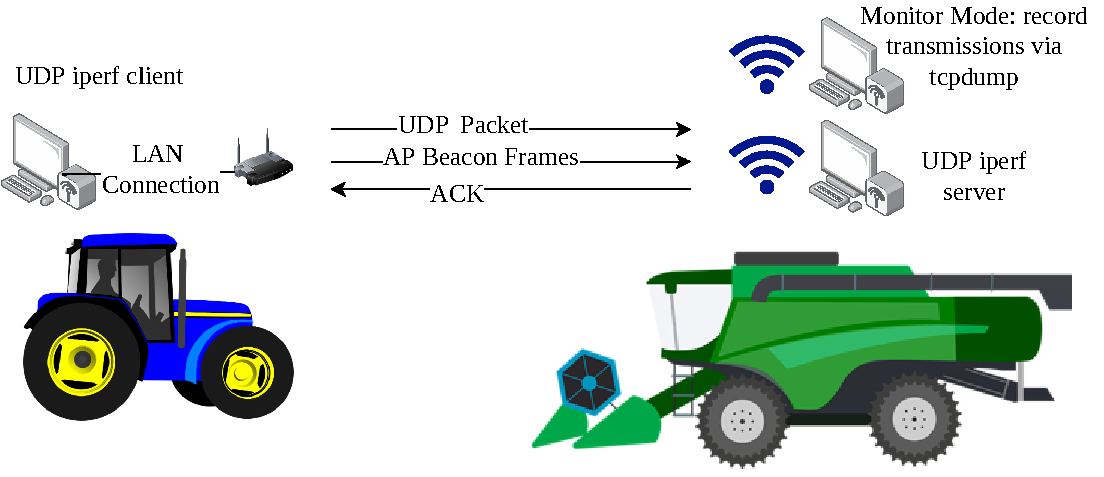
\includegraphics[width=0.8\textwidth]{figures/FieldExperimentwifi}
	\caption{Wi-Fi transmissions between the Wi-Fi \ac{AP} on the \acf{TM} and the Wi-Fi \ac{STA} on the \acf{CH}, which
	are recorded by a third Wi-Fi device in monitor mode on the \ac{CH}}
	\label{fig:fieldWifi}%
\end{figure}

The other UP Squared Board on the \ac{CH} uses the Wi-Fi card in the monitor mode and records every transmission in the \SI{5.6}{\giga\hertz} band using tcpdump \footnote{\url{https://www.tcpdump.org/}}.
Since the UP Squared board is placed next to the other board on the roof of the \ac{CH}, it can record the same signals the other board receives in the \ac{UDP} transmission.
The tcpdump records are in pcap - format, which can be analyzed using Wireshark\footnote{\url{https://www.wireshark.org/}}.
Using Wireshark, my plan is to identify possible retransmissions to calculate a \ac{PER}.
At the same time, the data contains the \ac{RSS} of each antenna and the physical layer parameters for every
transmission, allowing each transmission's robustness to be calculated as a function of the \ac{RSS} and the physical
layer configuration.

In order to get insights on the robustness of using the different frequency bands, the frequency channels for a \ac{BW} of \SI{20}{\mega\hertz} in \autoref{tab:fieldChannels} are configured.
To be able to calculate the means and standard deviations of the result for every configuration, the experiment is repeated \num{5} times for each channel,
which means that the tractor drives \num{5} times the same path, which is displayed in \autoref{fig:fieldDrive}.

\begin{table}[H]
	\centering
	\begin{tabular}{>{\centering}p{2cm}p{4cm}p{4cm}}
		\toprule
		\ac{BW} & Channel number \SI{2.4}{\giga\hertz} & Channel number \SI{5}{\giga\hertz}\\
		\midrule
		\SI{20}{\mega\hertz} & \num{1}&
		\num{100} \\
		\SI{40}{\mega\hertz} &
		\num{3}
		& \num{102} \\
		\SI{80}{\mega\hertz} &
		- & \num{106} \\
		\bottomrule
	\end{tabular}
	\caption{Frequency channel numbers for \SI{2.4}{\giga\hertz} and \SI{5}{\giga\hertz} for the different \acfp{BW} of the IEEE 802.11 standard \cite{ieee_standard_2021ax}, which can be used for
	outdoor communication \cite{freq_plan_24G}, \cite{freq_plan_5G} and can be configured in the Milesight Industrial Router UR75 for
	the field experiments.}
	\label{tab:fieldChannels}
\end{table}

\section{Trial Run}

To ensure that the experiment setup worked, I did a trial run and I got the data I needed as expected.
I mounted the Wi-Fi devices on the \ac{TM} and the \ac{CH} as shown in \autoref{fig:trailrunPositions} and
started the iperf3 client and server on the \ac{CH} and the \ac{TM} respectively.
During the trial run, the machines kept the same positions in a yard at the university.
To vary the recorded \ac{RSS}, I simultaneously moved the Wi-Fi antennas of the Wi-Fi devices on the \ac{CH} to
different positions.
I varied the used \ac{BW} of the \ac{AP} between \SIrange{20}{80}{\mega\hertz} in reference to \autoref{tab:fieldChannels}.
\begin{figure}[H]%
   \centering
   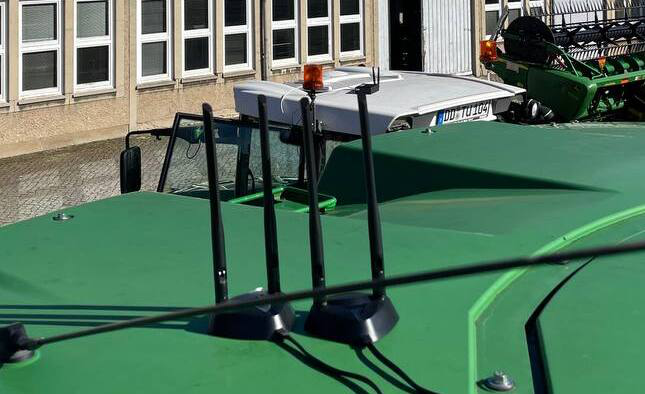
\includegraphics[width=0.5\textwidth]{figures/trainRun}
   \caption{Position of the Wi-Fi Devices on the \ac{TM} and the \ac{CH} during the trialrun}
   \label{fig:trailrunPositions}%
\end{figure}
The trial run was partly successful.
The monitoring Wi-Fi device blocked any try to configure monitoring channels with higher \ac{BW}s than \SI{20}{\mega\hertz}.
Therefore, I could only record data for a \ac{BW} of \SI{20}{\mega\hertz}.

The recorded data contains \ac{RSS}, physical layer configuration and MAC layer information of every received packet.
This can be used to find shadowing and fading effects, which may occur in the corn harvest scenario.

The recorded data was filtered to contain only the \ac{UDP} packets sent by the iperf3 client on the \ac{TM}
and displayed in \autoref{fig:trailrunIperf}.
It is visible that the Wi-Fi rate manager on the Milesight Industrial Router UR75 does not use \ac{STBC} and varies
the \ac{MCS} between \numrange{5}{8} and the \ac{GI} between \SIrange{400}{800}{\nano\second}.
Due to moving the antennas, the \ac{RSS} varies until I placed the antennas at a suitable fixed position at the end of the trial run.
As soon as the \ac{RSS} drops significantly at around \SIrange{25}{50}{\second}, the Wi-Fi rate manager switches to a lower \ac{MCS} and a longer
\ac{GI} to increase the transmission's robustness and reduce the retransmissions, which are indicated by the retry flag in the \ac{UDP} packet.

\begin{figure}[]%
   \centering
   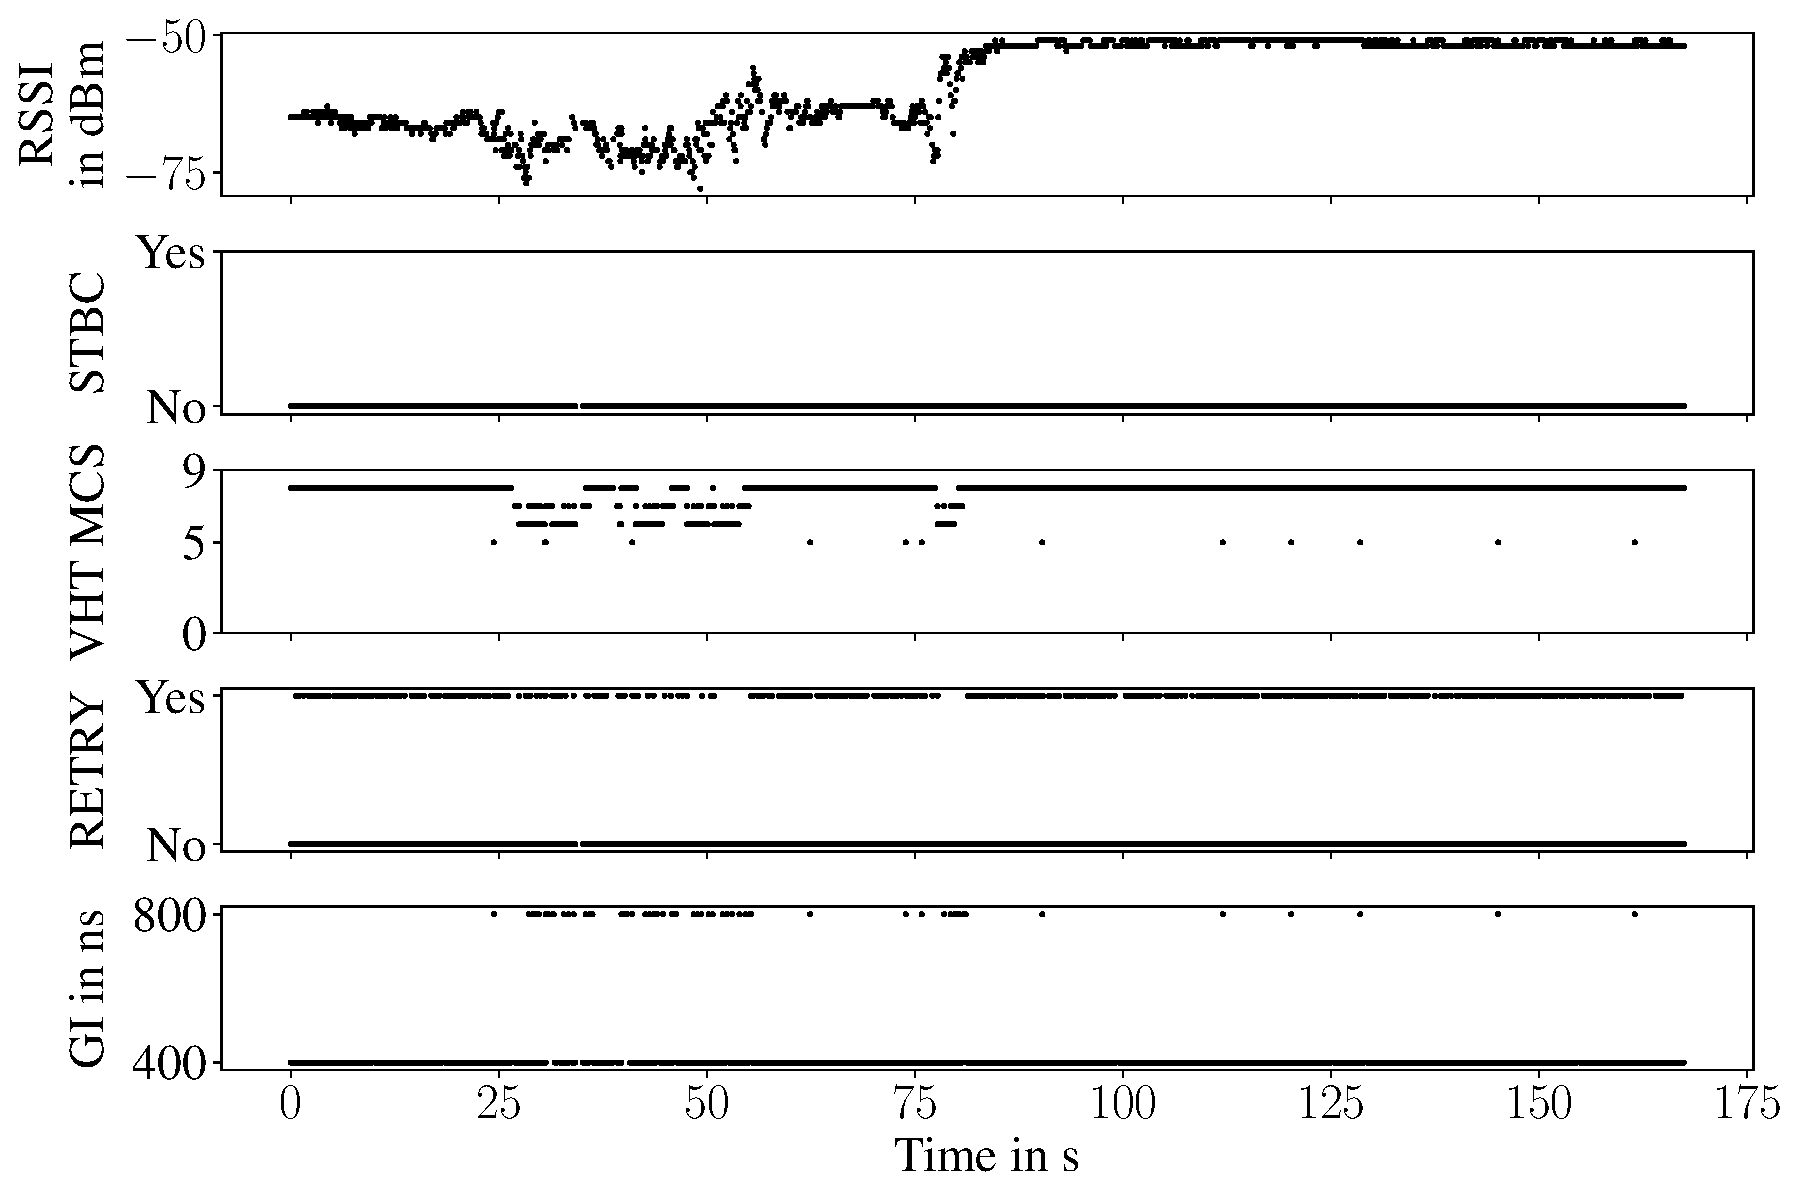
\includegraphics[width=0.95\textwidth]{figures/wireless5_144}
   \caption{All data transmissions between the Wi-Fi \acf{AP} on the \acf{TM} and the Wi-Fi \ac{STA} on the \acf{CH} in a trial run,
   which were initiated by the iperf3 client on the \acf{TM}}
   \label{fig:trailrunIperf}%
\end{figure}

The trial run took place in a yard at the university, where shadowing and fading effects due to buildings, trees, and agricultural machines are
expected.
The university ran other Wi-Fi networks, which may have interfered with my Wi-Fi network.
Therefore, many packets can get lost due to interference, shadowing or fading.

Every \ac{UDP} packet contains a sequence number to identify the packet.
If the packet is a retransmission, the packet contains the retry flag
with the same sequence number and data of the original transmission.
In general, \SI{25}{\percent} of received \ac{UDP} data packets contained retry flags.
This cannot be transferred to the \ac{PER} directly,
as it is unknown how many transmissions were sent by the iperf3 client and were lost due to interference, shadowing or fading.
To calculate the \ac{PER}, an additional Wi-Fi monitoring device next to the Wi-Fi router on the \ac{TM} is needed to record all
outgoing transmissions of the iperf3 client.
The \ac{PER} can then be calculated as the ratio of every successfully received \ac{UDP} packet to the number of transmitted \ac{UDP} packets.

Alternatively, retransmissions could be disabled as \textcite{klingler_agriculture_2018} did in their experiments.
Then every packet, which is missing in the sequence of received packets, is counted as a lost packet.
But the user interface of the Milesight Industrial Router UR75 has no option to disable retransmissions.

It is notable that the Wi-Fi rate manager on the Milesight Industrial Router UR75 always tries to use two spatial streams, the highest \ac{MCS} and the shortest \ac{GI} possible,
which results in the highest theoretical data rate.
For the \ac{BW} of \SI{20}{\mega\hertz}, the highest \ac{MCS} is \num{8} and the shortest \ac{GI} is \SI{400}{\nano\second} \cite{ieee_standard_2020}.
This translates to a theoretical data rate of \SI{173.3}{\mega\bit\per\second}, which is overdimensioned for the \ac{UDP} data packet rate of \SI{100}{\byte}
every \SI{100}{\milli\second}.
Additionally, the communication is less robust, which results in the high percentage of \SI{25}{\percent} of known retransmissions.

In the end, I could not conduct the proposed field experiments due to the rainy weather in the last \num{3} month of working period, which led to very wet agricultural fields.

\section{Wi-Fi Range Measurements}
Instead, I conducted a range measurement in an outdoor environment on an abandoned airfield near Mahlwinkel (52°23'17.9"N 11°50'35.4"E) in Saxony-Anhalt, Germany,
which can be seen in \autoref{fig:rangeEnvironment}.
The airfield was surrounded by grassland, wind turbines, a solar park and forests, which describe a typical environment for agricultural machines.
\begin{figure}[H]%
   \centering
   \includegraphics[width=0.6\textwidth]{figures/rangeMeasurementEnvironment}
   \caption{Airfield near Mahlwinkel (52°23'17.9"N 11°50'35.4"E) in Saxony-Anhalt, Germany, where I conducted the range measurements}
   \label{fig:rangeEnvironment}%
\end{figure}

I set up the Wi-Fi devices according to the setup above, where I replaced the \ac{CH} with a \SI{4}{\metre} wooden antenna mast and
the \ac{TM} with a roof extension on top of a car rack to reach a height of \SI{4}{\metre}.
The setup is shown in \autoref{fig:rangemeasurementSetup}.
\begin{figure}[]%
   \centering
   \includegraphics[width=0.6\textwidth]{figures/rangeMeasurementSetup}
   \caption{Setup of the Wi-Fi devices for the range measurements, which I mounted on wooden antenna masts to reach a height of \SI{4}{\metre}, the
   maximum allowed height of agricultural machines in Germany}
   \label{fig:rangemeasurementSetup}%
\end{figure}

The two Wi-Fi devices are mounted on the wooden antenna mast and were configured to run the iperf3 server and the monitoring mode.
I connected a \ac{GPS} receiver to the monitoring device and recorded the static position of the wooden antenna mast.
The wooden extension on top of the car rack carried the Wi-Fi router with the iperf3 client and an \ac{GPS} receiver to record the car's position every
second.

I place the Wi-Fi devices on the wooden antenna mast at one end of the airfield (52°23'17.8"N 11°50'41.7"E)
and drove the car with a speed of around \SI{10}{\kilo\metre\per\hour} (\SI{2.78}{\kilo\metre\per\hour}) the other end
of the airfield (52°23'17.8"N 11°50'29.7"E). Meanwhile, the iperf3 application exchanged \SI{100}{\byte} \ac{UDP} packets every
\SI{100}{\milli\second}.
Every Wi-fi transmission, which was received by the monitoring device, was recorded.
The iperf3 application ran while I drove away and back to the starting point.
I repeated this procedure three times to get a reliable result.

As I started the iperf3 client after the monitoring device, the first \ac{UDP} packets were recorded and used as a time reference to
synchronize the \ac{GPS} data of the car and the monitoring device.
I also used the recorded GPS time stamps to synchronize the recorded Wi-Fi transmissions with the \ac{GPS} logs.

\begin{figure}[]%
   \centering
   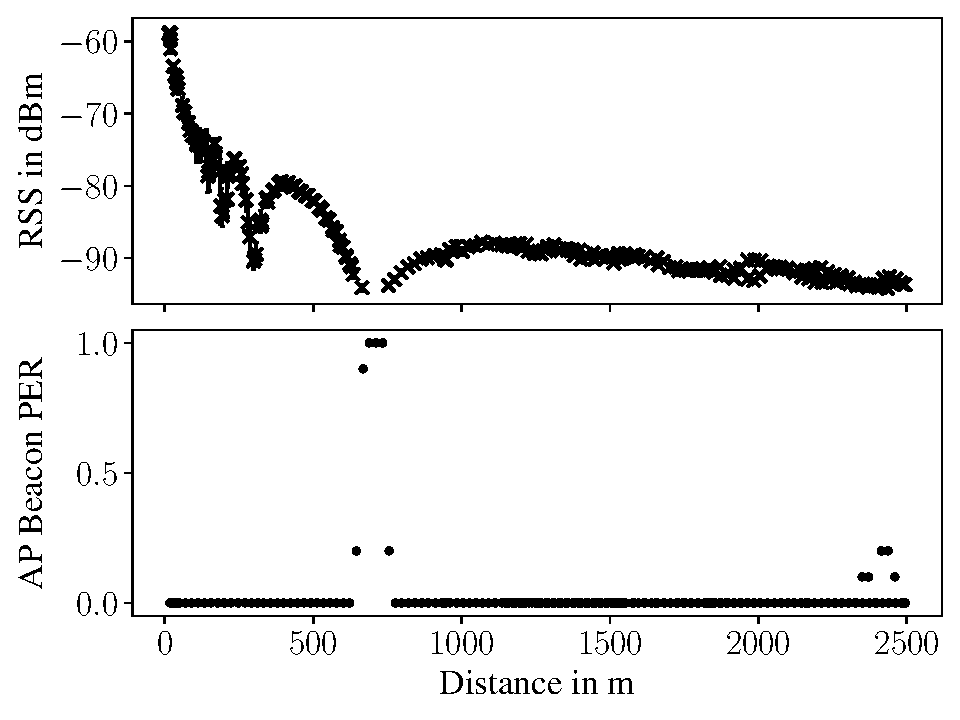
\includegraphics[width=0.8\textwidth]{figures/rangeMeasurementResults2}
   \caption{Range measurement results of the Wi-Fi transmissions on the airfield near Mahlwinkel (52°23'17.9"N 11°50'35.4"E) in Saxony-Anhalt, Germany}
   \label{fig:rangemeasurementResults}%
\end{figure}

The range measurement results are shown in \autoref{fig:rangemeasurementResults}.
I received Wi-Fi transmissions up to a distance of \SI{2.5}{\kilo\metre},
which equals the length of the airfield.

The \ac{RSS} values reflect a typical two-ray ground reflection model, where the ground reflection can be seen as a second ray,
which can cause destructive interference with the direct ray.
The destructive interference can be seen as the drops in the \ac{RSS} values.

At a distance of around \SIrange{650}{750}{\metre}, the \ac{RSS} values drop below the sensitivity of the Wi-Fi devices and
no Wi-Fi transmissions are received anymore.

This effect can also be detected in the \ac{PER} values of beacon frames.
The Milesight Industrial Router UR75 broadcasts every \SI{100}{\milli\second} the \ac{AP} beacon frame, which is used by Wi-Fi devices to
authenticate and associate with the \ac{AP}.
This beacon frame interval is defined in the recorded beacon frames and allows me to
calculate the \ac{PER} of the beacon frames as every \si{\second} \num{10} beacon frames should be received by the monitoring device.
The \ac{PER} of the beacon frames is shown in \autoref{fig:rangemeasurementResults} and indicates that no beacon frame was received at
a distance of around \SIrange{650}{750}{\metre}, because the \ac{RSS} values dropped below the sensitivity of the Wi-Fi devices.

Every beacon frame is transmitted in the IEEE 802.11a standard with a data rate of \SI{6}{\mega\bit\per\second}, which can also be received
by older Wi-Fi devices.
A data rate of \SI{6}{\mega\bit\per\second} refers to Binary \ac{PSK} modulation with a \ac{CR} of \nicefrac{1}{2} \cite{ieee_standard_1999}.
This \ac{MCS} and \ac{CR} combination is the most robust combination, which caused the low \ac{PER} values of the beacon frames over
the large communication range of up to \SI{2.5}{\kilo\metre}.
However, at the end of the communication range, the \ac{PER} values of the beacon frames
started to increase, because the \ac{RSS} values suffer more from fading effects and are not high enough to
to be sensed by the Wi-Fi devices.

The Wi-Fi rate manager on the Milesight Industrial Router UR75 used a \ac{VHT} \ac{MCS}0 for the \ac{UDP} data transmissions over this long communication distances, which also refers to a Binary \ac{PSK} modulation with a \ac{CR} of \nicefrac{1}{2}.
Additionally, it applied \ac{STBC} to increase the robustness of the Wi-Fi transmissions.

\section{Field Measurements Evaluation}

The achieved Wi-Fi transmission range may be dependent on the antenna height. \textcite{brinkhoff_characterization_2017} concluded that
the antenna height has a significant impact on the Wi-Fi transmission range.
They state, that the Wi-Fi transmission range increases
with the antenna height, because the Wi-Fi transmissions are less affected by obstacles and the Fresnel zone is less obstructed.
This effect is available until a maximum antenna height of \SI{50}{\metre} by the authors.

\textcite{krause_network_2021} performed simulations and measurements for network planning and coverage optimization of mobile campus networks for agricultural and construction site scenarios.
They assume tractor heights of \SI{3.5}{\meters} where an antenna can be mounted.
They conclude that higher antenna heights increase the fraction where a \ac{LOS} is available, resulting in
to a higher data rate and less shadowing.

In regard to antenna height, future field experiments should be conducted to find the optimal antenna height for agricultural machines.
Antennas heights can be built retractable and extendable to stay below the maximum allowed height of \SI{4}{\metre} for agricultural machines in Germany on
public roads and to be able to extend the antenna height to the optimal height for the Wi-Fi transmission range in agricultural fields.

\todo{Ground reflection coefficient beton grass,  permeability,  conductance, permittivity of grass, permittivity of concrete, permittivity of air, permittivity of water}

\ac{WIC} uses cases require reliable communication between the agricultural machines to exchange data
with each use case's specific required data rate, range, and latency.

The range measurements indicate that the Wi-Fi transmissions can be received up to a distance of \SI{2.5}{\kilo\metre},
which is sufficient to cover substantial agricultural fields.
However, Wi-Fi transmissions suffer from multipath, shadowing and fading effects, which can cause a large number of retransmissions,
when the physical layer configuration is oriented towards a high data rate instead of high robustness as it was
in the trial run.

As every used Wi-Fi device in the field experiment runs a Wi-Fi rate manager, which is responsible for the rate adaptation,
the influence of a particular physical layer parameter on the data goodput, robustness and latency can not be examined in the field experiment as no particular physical layer parameter can be set.
The Milesight Router is only capable of setting IEEE 802.11ac physical layer parameters, which don't include the new physical layer parameters of IEEE 802.11ax:
\ac{ER} mode, longer \ac{GI}s, \ac{HE}-\ac{MCS} \numrange{9}{11} or \ac{DCM}.

Taking \ac{DCM} as an example, the impact on the Wi-Fi receiver minimum input level sensitivity was mentioned in \autoref{fig:ReceiverSensitivityDCM}. \ac{DCM}
increases the robustness of the Wi-Fi transmissions and therefore allows a lower receiver minimum input level sensitivity to be used.

In the following chapter, I will analyze in simulations which physical layer
configurations are suitable for the agricultural environment to establish reliable communications,
which meets the data rate, range and latency requirements of Agricultural Platooning Services.
